\documentclass[a4paper]{article}
\usepackage[a4paper]{geometry}
\usepackage[utf8]{inputenc}

% Math packages
\usepackage{amsmath,amsfonts,amssymb}
\usepackage{array}

% Command control packages
\usepackage{ifthen}
\usepackage{ifpdf}

% Listings
\usepackage{listings}
\lstset{
  basicstyle=\ttfamily,
  columns=fullflexible,
  keepspaces=true,
  mathescape
}

% Tikz
\usepackage{tikz}


%%% Function arrows
\newcommand{\fun}{\rightarrow}

%%% Instruction formatting
\newcommand{\sourcecolortext}{blue}
\newcommand{\sourcecolor}[1]{\color{blue}}
\newcommand{\src}[1]{{\sourcecolor{} #1}}
\newcommand{\targetcolortext}{green}
\newcommand{\targetcolor}[1]{\color{green}}
\newcommand{\trg}[1]{{\targetcolor{} #1}}

\newcommand{\zinstr}[1]{#1}
\newcommand{\oneinstr}[2]{
  \ifthenelse{\equal{#2}{}}
  {\zinstr{#1}}
  {\zinstr{#1} \; #2}
}
\newcommand{\twoinstr}[3]{
  \ifthenelse{\equal{#2#3}{}}
  {\zinstr{#1}}
  {\zinstr{#1} \; #2 \; #3}
}
\newcommand{\threeinstr}[4]{
  \ifthenelse{\equal{#2#3#4}{}}
  {\zinstr{#1}}
  {\zinstr{#1} \; #2 \; #3 \; #4}
}

%%% Source language
% No arguments
\newcommand{\sfail}{\zinstr{\src{fail}}}
\newcommand{\shalt}{\zinstr{\src{halt}}}
\newcommand{\sreturn}{\zinstr{\src{return}}}

% One argument
\newcommand{\sjmp}[1]{\oneinstr{\src{jmp}}{#1}}
\newcommand{\spush}[1]{\oneinstr{\src{push}}{#1}}
\newcommand{\spop}[1]{\oneinstr{\src{pop}}{#1}}
\newcommand{\ssload}[1]{\oneinstr{\src{sload}}{#1}}

% Two arguments
\newcommand{\sjnz}[2]{\twoinstr{\src{jnz}}{#1}{#2}}
\newcommand{\sisptr}[2]{\twoinstr{\src{isptr}}{#1}{#2}}
\newcommand{\sgeta}[2]{\twoinstr{\src{geta}}{#1}{#2}}
\newcommand{\sgetb}[2]{\twoinstr{\src{getb}}{#1}{#2}}
\newcommand{\sgete}[2]{\twoinstr{\src{gete}}{#1}{#2}}
\newcommand{\sgetp}[2]{\twoinstr{\src{getp}}{#1}{#2}}
\newcommand{\sgetl}[2]{\twoinstr{\src{getl}}{#1}{#2}}
\newcommand{\smove}[2]{\twoinstr{\src{move}}{#1}{#2}}
\newcommand{\sstore}[2]{\twoinstr{\src{store}}{#1}{#2}}
\newcommand{\sload}[2]{\twoinstr{\src{load}}{#1}{#2}}
\newcommand{\slea}[2]{\twoinstr{\src{lea}}{#1}{#2}}
\newcommand{\scall}[2]{\twoinstr{\src{call}}{#1}{#2}}

% Three arguments
\newcommand{\srestrict}[3]{\threeinstr{\src{restrict}}{#1}{#2}{#3}}
\newcommand{\ssubseg}[3]{\threeinstr{\src{subseg}}{#1}{#2}{#3}}
\newcommand{\splus}[3]{\threeinstr{\src{plus}}{#1}{#2}{#3}}
\newcommand{\sminus}[3]{\threeinstr{\src{minus}}{#1}{#2}{#3}}

%%% Target language
% No arguments
\newcommand{\tfail}{\zinstr{\trg{fail}}}
\newcommand{\thalt}{\zinstr{\trg{halt}}}

% One argument
\newcommand{\tjmp}[1]{\oneinstr{\trg{jmp}}{#1}}

% Two arguments
\newcommand{\tjnz}[2]{\twoinstr{\trg{jnz}}{#1}{#2}}
\newcommand{\tisptr}[2]{\twoinstr{\trg{isptr}}{#1}{#2}}
\newcommand{\tgeta}[2]{\twoinstr{\trg{geta}}{#1}{#2}}
\newcommand{\tgetb}[2]{\twoinstr{\trg{getb}}{#1}{#2}}
\newcommand{\tgete}[2]{\twoinstr{\trg{gete}}{#1}{#2}}
\newcommand{\tgetp}[2]{\twoinstr{\trg{getp}}{#1}{#2}}
\newcommand{\tgetl}[2]{\twoinstr{\trg{getl}}{#1}{#2}}
\newcommand{\tmove}[2]{\twoinstr{\trg{move}}{#1}{#2}}
\newcommand{\tstore}[2]{\twoinstr{\trg{store}}{#1}{#2}}
\newcommand{\tload}[2]{\twoinstr{\trg{load}}{#1}{#2}}
\newcommand{\tlea}[2]{\twoinstr{\trg{lea}}{#1}{#2}}

% Three arguments
\newcommand{\trestrict}[3]{\threeinstr{\trg{restrict}}{#1}{#2}{#3}}
\newcommand{\tsubseg}[3]{\threeinstr{\trg{subseg}}{#1}{#2}{#3}}
\newcommand{\tplus}[3]{\threeinstr{\trg{plus}}{#1}{#2}{#3}}
\newcommand{\tminus}[3]{\threeinstr{\trg{minus}}{#1}{#2}{#3}}

%%% Domains
\newcommand{\plaindom}[1]{\mathrm{#1}}
\newcommand{\RegName}{\plaindom{RegisterName}}

\newcommand{\nats}{\mathbb{N}}

%%% Variables
\newcommand{\var}[1]{\mathit{#1}}
\newcommand{\rn}{\var{rn}}
\newcommand{\stk}{\var{stk}}

%%% Named registers
\newcommand{\pcreg}{\mathrm{pc}}
\newcommand{\rstk}{\mathrm{r}_\mathrm{stk}}
\newcommand{\rO}{\mathrm{r}_0}

%%% Permissions
\newcommand{\plainperm}[1]{\mathrm{#1}}
\newcommand{\rwlxo}{\plainperm{rwlxo}}
\newcommand{\rwlo}{\plainperm{rwlo}}
\newcommand{\rwl}{\plainperm{rwl}}
\newcommand{\rwxo}{\plainperm{rwxo}}
\newcommand{\rwo}{\plainperm{rwo}}
\newcommand{\rw}{\plainperm{rw}}
\newcommand{\rxo}{\plainperm{rxo}}
\newcommand{\ro}{\plainperm{ro}}
\newcommand{\readonly}{\plainperm{r}}
\newcommand{\noperm}{\plainperm{0}}
\newcommand{\nopermo}{\plainperm{0o}}
\newcommand{\enter}{\plainperm{e}}





%%% Braces
\newcommand{\comp}[1]{[#1]}

%%% Functions

\begin{document}
\section{The two capability machines}
\subsection{Domains}
\[
  \begin{array}{rcl}
    \{\pcreg,\rO,\rstk \} & \subseteq & \RegName
  \end{array}
\]

\subsection{Syntax}
The target machine is a simple capability machine with memory capabilities, local capabilities and enter capabilities. The syntax of the instructions of the target machine is defined as follows:
\[
\begin{array}{rcl}
n &\in & \nats \\
\trg{r} &\in &  \RegName  \src{\setminus \{\rO,\rstk\}}\\
\trg{\rn} &::= &  \trg{r} \mid n \\
\trg{i} &::= & \tfail \mid \thalt \mid \tjmp{\trg{r}} \mid \tjnz{\trg{r}}{\trg{\rn}} \mid \tisptr{\trg{r}}{\trg{r}} \mid \tgeta{\trg{r}}{\trg{r}} \mid \tgetb{\trg{r}}{\trg{r}} \mid \\
      & &  \tgete{\trg{r}}{\trg{r}}\mid \tgetp{\trg{r}}{\trg{r}} \mid \tgetl{\trg{r}}{\trg{r}} \mid \tmove{\trg{r}}{\trg{\rn}} \mid \tstore{\trg{r}}{\trg{r}} \mid\\
      & &  \tload{\trg{r}}{\trg{r}} \mid \tlea{\trg{r}}{\trg{\rn}} \mid \trestrict{\trg{r}}{\trg{r}}{\trg{\rn}} \mid \tsubseg{\trg{r}}{\trg{\rn}}{\trg{\rn}} \mid \\
      & & \tplus{\trg{r}}{\trg{\rn}}{\trg{\rn}} \mid \tminus{\trg{r}}{\trg{\rn}}{\trg{\rn}}
\end{array}
\]
Where the \sourcecolortext{} only applies for the source language which we define below.

The source machine is also a capability machine with memory capabilities, local capabilities and enter capabilities. Unlike the target machine, the source machine is going to have a built in stack. The syntax of the source machine language is as follows:
\[
  \begin{array}{rcl}
    n & \in & \nats \\
    \src{r} &\in &  \RegName \setminus \{\rO,\rstk\}\\
    \src{\rn} &::= & \src{r} \mid n \\
    \src{i} & ::= &  \trg{i} \mid \spop{\src{r}} \mid \spush{\src{\rn}} \mid \ssload{\src{\rn}} \mid \scall{\src{r}}{\src{\rn}} \mid \sreturn
  \end{array}
\]
There are two syntactic differences between the source language and the target language: (1) The source language does not permit register names $\rO$ and $\rstk$ to be used because they will play a special role in the compilation scheme. (2) The source language has explicit call/return instructions as well as the stack manipulation instructions $\spop{}$, $\spush{}$, $\ssload{}$, and $\scall{}{}$. We will define the semantic of these below.

\subsection{Permissions}


\begin{figure}[!h]
  \centering
  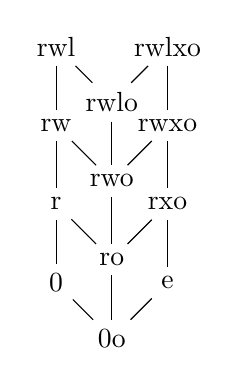
\begin{tikzpicture}[main node/.style={}]
    \node[main node] (7) {$\rwlxo$};
    \node[main node] (1) [below of=7] {$\rwxo$};
    \node[main node] (2) [below of=1] {$\rxo$};
    \node[main node] (3) [below of=2] {$\enter$};

    \node[main node] (9) [below left of=7] {$\rwlo$};
    \node[main node] (10) [below of=9] {$\rwo$};
    \node[main node] (11) [below of=10] {$\ro$};
    \node[main node] (12) [below of=11] {$\nopermo$};

    \node[main node] (8) [above left of=9] {$\rwl$};
    \node[main node] (4) [below of=8] {$\rw$};
    \node[main node] (5) [below of=4] {$\readonly$};
    \node[main node] (6) [below of=5] {$\noperm$};


    \path[every node/.style={font=\sffamily\small}]
    (7) edge (1)
    (8) edge (4)
    (1) edge (2)
    (2) edge (3)
    (4) edge (5)
    (5) edge (6)

    (9) edge (10)
    (10) edge (11)
    (11) edge (12)

    (9) edge (7)
    (10) edge (1)
    (11) edge (2)
    (12) edge (3)

    (9) edge (8)
    (10) edge (4)
    (11) edge (5)
    (12) edge (6);
  \end{tikzpicture}

  \caption{Permission hierarchy}
  \label{fig:perm-hier}
\end{figure}

\subsection{Compiler}
\[
\comp{\cdot} : \src{i}^* \fun \trg{i}^*
\]
\clearpage
\section{Examples}
\subsection{Capabilitiy opacity}
The following pseudo program demonstrates the need of opaque capabilities. If we assume a system with no opaque capabilities, then the following programs break compiler corretness
\begin{lstlisting}[basicstyle=\sourcecolor{}\ttfamily] 
p1 ::= if r1 is length 2 then
         call r1 with the following callback in r5:
           {put $\textit{\texttt{diverging}}$ closure in r2;
            return};
         halt
       else diverge

p2 ::= if r1 is length 2 then
         call r1 with the following callback in r5:
           {put $\textit{\texttt{terminating}}$ closure in r2;
            return};
         halt
       else diverge
\end{lstlisting}
The diverging closure could just contain $\sjmp{\pcreg}$, which diverges. The terminating closure could just be $\sreturn$.

The context with $r1$ as an executable capability pointing to:
\begin{lstlisting}
$\scall{r5}{0}$
$\sjmp{r5}$
\end{lstlisting}
distinguishes the two contexts, but two instructions are not enough to do the same at the target level. We would not have enough instructions to set up a proper return pointer for the compiled return to use.

\clearpage
\section{Back translation}
We want to do the back translation by interpreting the programs.
\end{document}